\documentclass[12pt]{article}
\usepackage{fullpage}

\usepackage{graphicx}        % Enable graphics commands
\usepackage{lscape}		% Enable landscape with \begin{landscape} until \end{landscape}
\usepackage{natbib}			% Enable citation commands \citep{}, \citet{}, etc.
\bibpunct{(}{)}{;}{a}{}{,}		% Formatting for in-text citations
\usepackage{setspace}		% Enable double-spacing with \begin{spacing}{2} until \end{spacing}.
\usepackage[utf8]{inputenc} 	% Enable utf8 characters, i.e., accents without coding--just type them in.
\usepackage[english]{babel}	% English hyphenation and alphabetization.  Other languages available.
\usepackage{dcolumn}        % For decimal-aligned stargazer output.
\usepackage[colorlinks=true, urlcolor=blue, citecolor=black, linkcolor=black]{hyperref} % Include hyperlinks with the \url and \href commands.
\setlength{\tabcolsep}{1pt}	% Make tables slightly narrower by reducing space between columns.

\renewcommand\floatpagefraction{.9}	% These commands allow larger tables and graphics to fit
\renewcommand\topfraction{.9}		% on a page when default settings would complain.
\renewcommand\bottomfraction{.9}
\renewcommand\textfraction{.1}
\setcounter{totalnumber}{50}
\setcounter{topnumber}{50}
\setcounter{bottomnumber}{50}

\newcommand{\R}{\textsf{R}~}        %This creates the command \R to typeset the name R correctly.

%\usepackage[left=1in, right=1in]{geometry}	%Turn footnotes into endnotes (commented out).
%\renewcommand{\footnotesize}{\normalsize}	
%\usepackage{endnotes}
%\renewcommand{\footnote}{\endnote}
%\renewcommand{\section}{\subsection}

\usepackage{Sweave}
\begin{document}
\Sconcordance{concordance:Exam.tex:Exam.Rnw:%
1 30 1 1 0 13 1 1 3 2 0 1 1 15 0 1 2 3 1 11 0 1 2 6 1 1 2 4 0 1 7 28 0 %
1 2 4 1 1 2 5 0 1 3 1 6 35 0 1 3 6 1 1 2 1 0 2 1 6 0 1 1 6 0 1 1 6 0 1 %
1 7 0 1 2 6 1 1 2 4 0 1 2 1 7 31 0 1 2 5 1 1 2 1 0 2 1 3 0 1 2 1 7 35 0 %
1 2 5 1 1 47 6 0 1 3 17 1 1 12 10 0 1 2 1 1 6 0 1 2 1 22 20 0 1 7 5 0 1 %
3 1 0 1 2 65 0 1 2 20 0 1 1 1 5 6 0 1 5 1 3 2 0 1 5 3 0 1 6 4 0 1 2 1 1 %
54 0 1 1 1 23 21 0 1 2 3 1 1 7 8 0 1 2 1 4 26 1 1 26 25 0 2 2 66 0 1 2 %
2 1 1 2 21 0 1 1 21 0 1 2 4 1}


\pagestyle{empty}

\begin{center}
{\Large \textbf{POLI 5003: Exam}}
\end{center}

\textbf{Directions.}  Making sure not only to provide output of the requested analyses but also to describe your results textually, please use these data to answer the following questions.  You may consult any materials you choose, but please do not discuss the exam with anyone else; it is to be your work alone.  Please submit your \verb+.Rnw+ file via ICON Dropbox within 48 hours of downloading the exam materials.\\

In the included dataset \verb+press.dta+, the variable \verb+press_free+ is the Press Freedom Index compiled by Reporters Without Borders for countries around the world in the year 2008.  (To make the variable more intuitive, it was reversed from the RWB scaling so that high values represent more press freedom.)  Suppose we are interested in the effect of international conflict on governments' respect for freedom of the press.  The variable \texttt{conflict} is the number of serious international conflicts (those that escalated to uses of force or outright war) in which each country had recently taken part according to the Correlates of War dataset.  


\begin{Schunk}
\begin{Sinput}
> # Setup
> needed.packages <- c("foreign", "stargazer", "ggplot2", "rstan")
> lapply(needed.packages, require, character.only=T)
\end{Sinput}
\begin{Soutput}
[[1]]
[1] TRUE

[[2]]
[1] TRUE

[[3]]
[1] TRUE

[[4]]
[1] TRUE
\end{Soutput}
\begin{Sinput}
> press <- read.dta("press.dta")
> var.labels <- attr(press,"var.labels")
> data.key <- data.frame(var.name=names(press),var.labels)
> data.key
\end{Sinput}
\begin{Soutput}
    var.name                              var.labels
1    country                                        
2 press_free                     Press Freedom Index
3   conflict      Serious Int'l Conflicts, 1998-2008
4        dem Democratic regime per Przeworski et al.
5     gdp_pc                   GDP per capita, $000s
\end{Soutput}
\end{Schunk}

\pagebreak
\subsection*{Part 1: Classical Linear Regression}

\begin{enumerate}
\item Does a simple regression support the hypothesis that countries that have been engaged in more conflicts have less respect for freedom of the press?  How do you know?  Describe the estimated effect of conflicts on press freedom.\\

\begin{Schunk}
\begin{Sinput}
> fit.1 <- lm(press_free ~ conflict, data=press)
\end{Sinput}
\end{Schunk}
% Table created by stargazer v.4.5.3 by Marek Hlavac, Harvard University. E-mail: hlavac at fas.harvard.edu
% Date and time: Mon, Mar 24, 2014 - 11:03:54 AM
\begin{table}[!htbp] \centering 
  \caption{Effect of Conflict on Press Freedom} 
  \label{} 
\begin{tabular}{@{\extracolsep{5pt}}lc} 
\\[-1.8ex]\hline 
\hline \\[-1.8ex] 
 & \multicolumn{1}{c}{\textit{Dependent variable:}} \\ 
\cline{2-2} 
\\[-1.8ex] & Press Freedom \\ 
\hline \\[-1.8ex] 
 Conflict & $-$1.072$^{**}$ \\ 
  & (0.540) \\ 
  & \\ 
 Constant & 77.398$^{***}$ \\ 
  & (2.195) \\ 
  & \\ 
\hline \\[-1.8ex] 
Observations & 142 \\ 
R$^{2}$ & 0.027 \\ 
Adjusted R$^{2}$ & 0.020 \\ 
Residual Std. Error & 21.365 (df = 140) \\ 
F Statistic & 3.936$^{**}$ (df = 1; 140) \\ 
\hline 
\hline \\[-1.8ex] 
\textit{Note:}  & \multicolumn{1}{r}{$^{*}$p$<$0.1; $^{**}$p$<$0.05; $^{***}$p$<$0.01} \\ 
\normalsize 
\end{tabular} 
\end{table} 
The table above reports results from a simple bivaraite regression of the press freedom measure on number of conflicts.  There appears to be a statistically significant relationship between the number of conflicts a country engages in and their relative press freedom score.  The more conflict, the less press freedom.  For each additional conflict experienced an estimated reduction of 1.072 in the press freedom measure occurs.  This relationship is significant at the .05 level.  So there appears to be a relationship between the two variables that is statistically significantly different from zero and is negative - there is support for the hypothesis.

\item Is the hypothesis supported when controls for domestic regime type (\verb+dem+) and GDP per capita (\verb+gdp_pc+) are introduced?  Use \verb+stargazer+ to present the results for both models in a neatly-formatted table.  (Recall that the file \verb+LaTeX_Example.Rnw+ in the course's GitHub directory provides an example of how to use \verb+stargazer+.) \\

\begin{Schunk}
\begin{Sinput}
> fit.2 <- lm(press_free ~ conflict + dem + gdp_pc, data=press)
> 
\end{Sinput}
\end{Schunk}

% Table created by stargazer v.4.5.3 by Marek Hlavac, Harvard University. E-mail: hlavac at fas.harvard.edu
% Date and time: Mon, Mar 24, 2014 - 11:03:54 AM
\begin{table}[!htbp] \centering 
  \caption{Effect of Conflict on Press Freedom} 
  \label{} 
\begin{tabular}{@{\extracolsep{5pt}}lcc} 
\\[-1.8ex]\hline 
\hline \\[-1.8ex] 
 & \multicolumn{2}{c}{\textit{Dependent variable:}} \\ 
\cline{2-3} 
\\[-1.8ex] & \multicolumn{2}{c}{Press Freedom} \\ 
\\[-1.8ex] & (1) & (2)\\ 
\hline \\[-1.8ex] 
 Conflict & $-$1.072$^{**}$ & $-$1.142$^{***}$ \\ 
  & (0.540) & (0.429) \\ 
  & & \\ 
 Regime Type &  & 22.193$^{***}$ \\ 
  &  & (2.922) \\ 
  & & \\ 
 GDP Per Capita &  & 0.272$^{***}$ \\ 
  &  & (0.076) \\ 
  & & \\ 
 Constant & 77.398$^{***}$ & 61.372$^{***}$ \\ 
  & (2.195) & (2.471) \\ 
  & & \\ 
\hline \\[-1.8ex] 
Observations & 142 & 142 \\ 
R$^{2}$ & 0.027 & 0.395 \\ 
Adjusted R$^{2}$ & 0.020 & 0.382 \\ 
Residual Std. Error & 21.365 (df = 140) & 16.965 (df = 138) \\ 
F Statistic & 3.936$^{**}$ (df = 1; 140) & 30.092$^{***}$ (df = 3; 138) \\ 
\hline 
\hline \\[-1.8ex] 
\textit{Note:}  & \multicolumn{2}{r}{$^{*}$p$<$0.1; $^{**}$p$<$0.05; $^{***}$p$<$0.01} \\ 
\normalsize 
\end{tabular} 
\end{table} 
The results presented above in Table 2 confirm our findings from Table 1: there is a statistically significant negative relationship between the number of conflicts a country engages in and their relative press freedom score.  In the second model, which includes control variables for regime type and GDP per capita, this relationship is even stronger.  The coefficient increases in both size and significance.  As expected, both regime type and GDP per capita have a statistically significant effect in the expected direction.  Notably, the adjusted R$^2$ value increases rather drastically when we include just these two control variables.  This means our second model is a better fit and explains a little bit more of the variance in the dependent variable.  Yes, the hypothesis is still supported when including these controls.


\pagebreak
\item Assess the substantive significance of the estimated effects of all three independent variables.  

\begin{Schunk}
\begin{Sinput}
> press.range <- apply(press[,3:5], 2, function(x) max(x) - min(x))
> max.effects <- press.range * fit.2$coef[2:4]
> max.effects
\end{Sinput}
\begin{Soutput}
 conflict       dem    gdp_pc 
-22.83342  22.19265  40.69851 
\end{Soutput}
\begin{Sinput}
> summary(press$gdp_pc)
\end{Sinput}
\begin{Soutput}
    Min.  1st Qu.   Median     Mean  3rd Qu.     Max. 
  0.1361   1.9420   7.1800  14.1300  20.4100 149.8000 
\end{Soutput}
\begin{Sinput}
> summary(press$conflict)
\end{Sinput}
\begin{Soutput}
   Min. 1st Qu.  Median    Mean 3rd Qu.    Max. 
  0.000   0.000   1.000   2.345   3.000  20.000 
\end{Soutput}
\begin{Sinput}
> table(press$conflict)
\end{Sinput}
\begin{Soutput}
 0  1  2  3  4  5  6  7  8  9 10 11 12 18 20 
48 38 14  8  7  7  3  6  5  1  1  1  1  1  1 
\end{Soutput}
\end{Schunk}

To assess the substnative significance of the estimated effects of all three independent variables I compared the maximum effect of each.  That is, I calculated what the estimated effect of going from the minimum value to the maximum value on each independent variable would be, while holding the other indepdendent variables constant.  The results, shown above, indicate that GDP per capita appears to have the greatest substantive effect on the dependent variable, press freedom.  This is partly attributable to the high amount of variation in the GDP per capita variable, illustrated in the summary statistics presented above as well. \\

These findings should be used carefully, however.  At first glance the summary statistics of the conflict variable do not raise any red flags.  However, looking at the frequency table of the variable, we can see that a large portion of our sample is clustered near the bottom zero and one values.  This creates a problem for our analysis.  The substantive effect of conflict is quite large, as moving from zero to the max (20) results in a reduction of 22.83 on the press freedom score.  However, very few countries experience more than 8 conflicts, there is a gap of no cases from 13-17, and, as mentioned earlier, most cases are clustered near the bottom of this scale.  Therefore, the estimated substantive effect presented above might not be that reliable.  In addition, although dem is the largest coefficient in our table above, we can see this is because it is dichotomous - the other variables in our model have greater effects when moving from the min to the max.

\item Suppose we think the responses of democracies and nondemocracies to conflict are different with regard to press freedom.  Is there support for this conditional hypothesis?  How do you know?\\

\begin{Schunk}
\begin{Sinput}
> fit.4 <- lm(press_free ~ conflict + dem + gdp_pc + conflict*dem, data=press)
\end{Sinput}
\end{Schunk}

% Table created by stargazer v.4.5.3 by Marek Hlavac, Harvard University. E-mail: hlavac at fas.harvard.edu
% Date and time: Mon, Mar 24, 2014 - 11:03:55 AM
\begin{table}[!htbp] \centering 
  \caption{Effect of Conflict on Press Freedom} 
  \label{} 
\begin{tabular}{@{\extracolsep{5pt}}lccc} 
\\[-1.8ex]\hline 
\hline \\[-1.8ex] 
 & \multicolumn{3}{c}{\textit{Dependent variable:}} \\ 
\cline{2-4} 
\\[-1.8ex] & \multicolumn{3}{c}{Press Freedom} \\ 
\\[-1.8ex] & (1) & (2) & (3)\\ 
\hline \\[-1.8ex] 
 Conflict & $-$1.072$^{**}$ & $-$1.142$^{***}$ & $-$2.568$^{***}$ \\ 
  & (0.540) & (0.429) & (0.750) \\ 
  Democracy &  & 22.193$^{***}$ & 17.436$^{***}$ \\ 
  &  & (2.922) & (3.541) \\ 
  GDP Per Capita &  & 0.272$^{***}$ & 0.260$^{***}$ \\ 
  &  & (0.076) & (0.075) \\ 
  Conflict * Democracy &  &  & 2.094$^{**}$ \\ 
  &  &  & (0.909) \\ 
  Constant & 77.398$^{***}$ & 61.372$^{***}$ & 64.728$^{***}$ \\ 
  & (2.195) & (2.471) & (2.835) \\ 
 \hline \\[-1.8ex] 
Observations & 142 & 142 & 142 \\ 
R$^{2}$ & 0.027 & 0.395 & 0.418 \\ 
Adjusted R$^{2}$ & 0.020 & 0.382 & 0.401 \\ 
\hline 
\hline \\[-1.8ex] 
\textit{Note:}  & \multicolumn{3}{r}{$^{*}$p$<$0.1; $^{**}$p$<$0.05; $^{***}$p$<$0.01} \\ 
\normalsize 
\end{tabular} 
\end{table} 
Yes, there does appear to be support for this conditional hypothesis.  I included an interaction term between conflict and regime type in the third model in Table 3, above.  There are several notable findings.  First, the interaction term is statistically significant at the .05 level.  How conflict affects democracies and how conflict affects non-democracies is statistically significantly different from zero.  That is, the conflict variable affects the two regime types in different ways.  The interaction term coefficient is telling us that there is indeed a different effect of conflict on press freedom for democracies than there is for non-democracies.  Looking to the conflict variable in model 3 above, we see that among non-democracies (when the dem variable equals zero) conflict has a statistically significant negative effect on relative press freedom scores.  For each conflict, non-democracies experience a 2.568 reduction in relative press freedom scores.

\pagebreak
\item Does conflict have a statistically significant effect on the press freedom of nondemocracies?  On that of democracies?  Report the estimated effect and $p$-value for each.\\

\begin{Schunk}
\begin{Sinput}
> press$non_dem[press$dem==0] <- 1
> press$non_dem[press$dem==1] <- 0
> fit.5 <- lm(press_free ~ conflict + non_dem + gdp_pc + conflict*non_dem, data=press)
\end{Sinput}
\end{Schunk}

% Table created by stargazer v.4.5.3 by Marek Hlavac, Harvard University. E-mail: hlavac at fas.harvard.edu
% Date and time: Mon, Mar 24, 2014 - 11:03:55 AM
\begin{table}[!htbp] \centering 
  \caption{Effect of Conflict on Press Freedom} 
  \label{} 
\begin{tabular}{@{\extracolsep{5pt}}lcccc} 
\\[-1.8ex]\hline 
\hline \\[-1.8ex] 
 & \multicolumn{4}{c}{\textit{Dependent variable:}} \\ 
\cline{2-5} 
\\[-1.8ex] & \multicolumn{4}{c}{Press Freedom} \\ 
\\[-1.8ex] & (1) & (2) & (3) & (4)\\ 
\hline \\[-1.8ex] 
 Conflict & $-$1.072$^{**}$ & $-$1.142$^{***}$ & $-$2.568$^{***}$ & $-$0.474 \\ 
  & (0.540) & (0.429) & (0.750) & (0.512) \\ 
  Democracy &  & 22.193$^{***}$ & 17.436$^{***}$ &  \\ 
  &  & (2.922) & (3.541) &  \\ 
  Non-Democracy &  &  &  & $-$17.436$^{***}$ \\ 
  &  &  &  & (3.541) \\ 
  GDP Per Capita &  & 0.272$^{***}$ & 0.260$^{***}$ & 0.260$^{***}$ \\ 
  &  & (0.076) & (0.075) & (0.075) \\ 
  Conflict * Democracy &  &  & 2.094$^{**}$ &  \\ 
  &  &  & (0.909) &  \\ 
  Conflict* Non-Democracy &  &  &  & $-$2.094$^{**}$ \\ 
  &  &  &  & (0.909) \\ 
  Constant & 77.398$^{***}$ & 61.372$^{***}$ & 64.728$^{***}$ & 82.164$^{***}$ \\ 
  & (2.195) & (2.471) & (2.835) & (2.580) \\ 
 \hline \\[-1.8ex] 
Observations & 142 & 142 & 142 & 142 \\ 
R$^{2}$ & 0.027 & 0.395 & 0.418 & 0.418 \\ 
Adjusted R$^{2}$ & 0.020 & 0.382 & 0.401 & 0.401 \\ 
\hline 
\hline \\[-1.8ex] 
\textit{Note:}  & \multicolumn{4}{r}{$^{*}$p$<$0.1; $^{**}$p$<$0.05; $^{***}$p$<$0.01} \\ 
\normalsize 
\end{tabular} 
\end{table} 
In Table 4 model 4 I simply reversed the dichotomous variable dem so that 1s are now 0s and vice-versa.  This changes the focus from democracies as a unit to non-democracies as a unit.  We see a statistically significant interaction term again, similar to the one in model 3.  However, the conflict variable is no long significant.  This means that for democracies (when nondem is equal to zero), conflict does not seem to have a statistically significant effect on press freedom.  For non-democracies, this does not appear to be true.  Since the interaction term is significant in both models we can conclude that there is indeed a difference in the way the conflict variable influences press freedom by regime type.  By looking at the conflict variable in each model we can see that conflict has a statistically significant negative effect for non-democracies, but does not appear to have an effect on democracies.  

\pagebreak
\item Suppose we were really more interested the difference in press freedom between democracies and nondemocracies.  What effect does conflict have on this difference? Your answer should include a graph generated using the \verb+interplot+ function from the course's GitHub page.\\

\begin{Schunk}
\begin{Soutput}
  dem       coef         ub        lb
1   0 -2.6011224 -1.0444998 -4.121163
2   1 -0.4755399  0.6186037 -1.492885
\end{Soutput}
\end{Schunk}

\begin{figure}[htbp] 
  \caption{Conditional Effect of Democracy by Level of International Conflict}
  \label{F:dem}
  \begin{center}
%   Uncomment the following line once you've generated the graph
    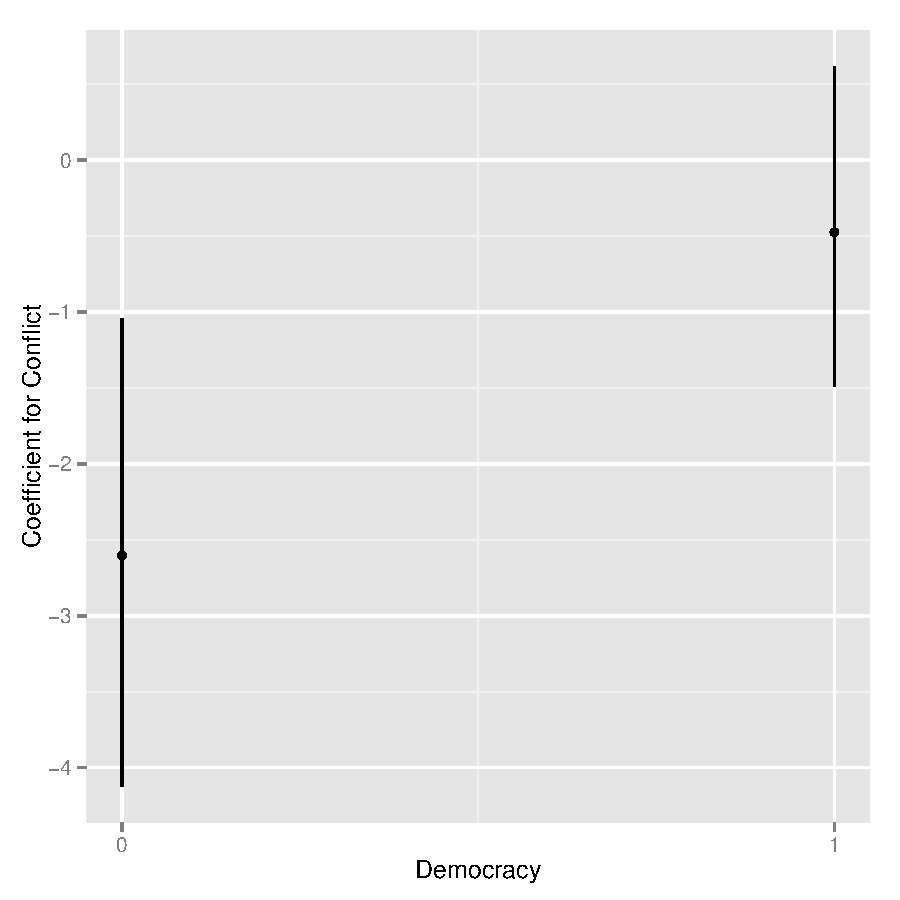
\includegraphics[width=5.25in]{Exam-f1.pdf}
  \end{center}
\end{figure}

Figure 1 shows how the effect of conflict on relative press freedom scores is conditioned by the regime type of a country.  The graph plots the coefficient for conflict and its confidence interval for both democracies (1) and non-democracies (0).  For democracies we see a confidence interval containing zero; conflict does not appear to have a statistically significant effect on press freedom that is different from zero.  For non-democracies, however, we see a confidence interval that is solidly in negative numbers.  From this graph we can conclude that the effect of conflict on press freedom varies by regime type.


\pagebreak
\subsection*{Part 2: Bayesian Linear Regression}

\item Consider again the unconditional hypothesis that countries that have been engaged in a larger number of serious international conflicts will evince less respect for freedom of the press, even when taking into account their regime type and their GDP per capita.  Does the posterior of a Bayesian linear regression with uninformative uniform priors support this hypothesis?

\begin{Schunk}
\begin{Sinput}
> ######################
> # Requiried packages #
> ######################
> 
> ipak <- function(pkg){
+     new.pkg <- pkg[!(pkg %in% installed.packages()[, "Package"])]
+     if (length(new.pkg)) 
+         install.packages(new.pkg, dependencies = TRUE)
+     sapply(pkg, require, character.only = TRUE)
+ }
> packages <- c("ggplot2", "RCurl", "MCMCpack", "inline", "Rcpp")
> ipak(packages)
\end{Sinput}
\begin{Soutput}
 ggplot2    RCurl MCMCpack   inline     Rcpp 
    TRUE     TRUE     TRUE     TRUE     TRUE 
\end{Soutput}
\begin{Sinput}
> require(rstan)
> #define the model
> pressfree.code <- '
+     data {
+         int<lower=0> N;
+         vector[N] press_free;
+         vector[N] conflict;
+         vector[N] dem;
+         vector[N] gdp_pc;
+     }
+     parameters {                
+         real beta1;             // coef for constant (default prior is uniform, i.e., noninformative)
+         real beta2;             // coef for stategini
+         real beta3;
+         real beta4;
+         real<lower=0> sigma;
+     }
+     model {
+         press_free ~ normal(beta1 + beta2 * conflict + beta3 * dem +
+                              beta4 * gdp_pc, sigma);
+     }
+ '
> # put data into expected format
> press.data <- list(N = nrow(press), 
+                    press_free = press$press_free, 
+                    conflict = press$conflict, 
+                    dem = press$dem, 
+                    gdp_pc = press$gdp_pc)
> # Now we can run it
> set.seed(324)
> m1.stan <- stan(model_code = pressfree.code, data = press.data, 
+                 iter = 10000, chains = 3)
\end{Sinput}
\begin{Soutput}
TRANSLATING MODEL 'pressfree.code' FROM Stan CODE TO C++ CODE NOW.
COMPILING THE C++ CODE FOR MODEL 'pressfree.code' NOW.
cygwin warning:
  MS-DOS style path detected: C:/PROGRA~1/R/R-30~1.2/etc/x64/Makeconf
  Preferred POSIX equivalent is: /cygdrive/c/PROGRA~1/R/R-30~1.2/etc/x64/Makeconf
  CYGWIN environment variable option "nodosfilewarning" turns off this warning.
  Consult the user's guide for more details about POSIX paths:
    http://cygwin.com/cygwin-ug-net/using.html#using-pathnames
C:/Users/kellengracey/Documents/R/win-library/3.0/rstan/include//stansrc/stan/agrad/rev/var_stack.hpp:49:17: warning: 'void stan::agrad::free_memory()' defined but not used [-Wunused-function]
C:/Users/kellengracey/Documents/R/win-library/3.0/rstan/include//stansrc/stan/agrad/rev/chainable.hpp:87:17: warning: 'void stan::agrad::set_zero_all_adjoints()' defined but not used [-Wunused-function]
SAMPLING FOR MODEL 'pressfree.code' NOW (CHAIN 1).

Iteration:    1 / 10000 [  0%]  (Warmup)
Iteration: 1000 / 10000 [ 10%]  (Warmup)
Iteration: 2000 / 10000 [ 20%]  (Warmup)
Iteration: 3000 / 10000 [ 30%]  (Warmup)
Iteration: 4000 / 10000 [ 40%]  (Warmup)
Iteration: 5000 / 10000 [ 50%]  (Warmup)
Iteration: 6000 / 10000 [ 60%]  (Sampling)
Iteration: 7000 / 10000 [ 70%]  (Sampling)
Iteration: 8000 / 10000 [ 80%]  (Sampling)
Iteration: 9000 / 10000 [ 90%]  (Sampling)
Iteration: 10000 / 10000 [100%]  (Sampling)
Elapsed Time: 1.328 seconds (Warm-up)
              1.182 seconds (Sampling)
              2.51 seconds (Total)

SAMPLING FOR MODEL 'pressfree.code' NOW (CHAIN 2).

Iteration:    1 / 10000 [  0%]  (Warmup)
Iteration: 1000 / 10000 [ 10%]  (Warmup)
Iteration: 2000 / 10000 [ 20%]  (Warmup)
Iteration: 3000 / 10000 [ 30%]  (Warmup)
Iteration: 4000 / 10000 [ 40%]  (Warmup)
Iteration: 5000 / 10000 [ 50%]  (Warmup)
Iteration: 6000 / 10000 [ 60%]  (Sampling)
Iteration: 7000 / 10000 [ 70%]  (Sampling)
Iteration: 8000 / 10000 [ 80%]  (Sampling)
Iteration: 9000 / 10000 [ 90%]  (Sampling)
Iteration: 10000 / 10000 [100%]  (Sampling)
Elapsed Time: 1.248 seconds (Warm-up)
              1.259 seconds (Sampling)
              2.507 seconds (Total)

SAMPLING FOR MODEL 'pressfree.code' NOW (CHAIN 3).

Iteration:    1 / 10000 [  0%]  (Warmup)
Iteration: 1000 / 10000 [ 10%]  (Warmup)
Iteration: 2000 / 10000 [ 20%]  (Warmup)
Iteration: 3000 / 10000 [ 30%]  (Warmup)
Iteration: 4000 / 10000 [ 40%]  (Warmup)
Iteration: 5000 / 10000 [ 50%]  (Warmup)
Iteration: 6000 / 10000 [ 60%]  (Sampling)
Iteration: 7000 / 10000 [ 70%]  (Sampling)
Iteration: 8000 / 10000 [ 80%]  (Sampling)
Iteration: 9000 / 10000 [ 90%]  (Sampling)
Iteration: 10000 / 10000 [100%]  (Sampling)
Elapsed Time: 1.185 seconds (Warm-up)
              1.27 seconds (Sampling)
              2.455 seconds (Total)
\end{Soutput}
\begin{Sinput}
> print(m1.stan)
\end{Sinput}
\begin{Soutput}
Inference for Stan model: pressfree.code.
3 chains, each with iter=10000; warmup=5000; thin=1; 
post-warmup draws per chain=5000, total post-warmup draws=15000.

        mean se_mean  sd   2.5%    25%    50%    75%  97.5% n_eff Rhat
beta1   61.4       0 2.5   56.5   59.7   61.4   63.1   66.4  6244    1
beta2   -1.2       0 0.4   -2.0   -1.4   -1.1   -0.9   -0.3  8258    1
beta3   22.2       0 3.0   16.3   20.3   22.3   24.2   28.0  7430    1
beta4    0.3       0 0.1    0.1    0.2    0.3    0.3    0.4  8560    1
sigma   17.1       0 1.0   15.2   16.4   17.1   17.8   19.3  9258    1
lp__  -470.7       0 1.6 -474.9 -471.6 -470.4 -469.6 -468.6  4693    1

Samples were drawn using NUTS(diag_e) at Mon Mar 24 11:04:40 2014.
For each parameter, n_eff is a crude measure of effective sample size,
and Rhat is the potential scale reduction factor on split chains (at 
convergence, Rhat=1).
\end{Soutput}
\begin{Sinput}
> m1.stan.sim <- as.data.frame(m1.stan)
> b.conflict.plot <- qplot(m1.stan.sim$beta2, geom="density") + 
+     xlab("Coefficient of Conflict") + 
+     ylab("Density of Posterior Distribution") +
+     theme_bw()
\end{Sinput}
\end{Schunk}

\begin{Schunk}
\begin{Sinput}
> # Graph regression results
> press2 <- press
> # Standardize continuous IVs by dividing by 2 s.d.s (per Gelman (2008))
> for (iv in 5:5) {
+     press2[,iv] <- press2[,iv]/(2*sd(press2[,iv]))
+ }
> press2.data <- list(N = nrow(press2), 
+                     press_free = press2$press_free, 
+                     conflict = press2$conflict,
+                     dem = press2$dem, 
+                     gdp_pc = press2$gdp_pc)
> set.seed(324)
> m1.stan2 <- stan(fit=m1.stan, data=press2.data, iter = 10000, chains = 3)
\end{Sinput}
\begin{Soutput}
SAMPLING FOR MODEL 'pressfree.code' NOW (CHAIN 1).

Iteration:    1 / 10000 [  0%]  (Warmup)
Iteration: 1000 / 10000 [ 10%]  (Warmup)
Iteration: 2000 / 10000 [ 20%]  (Warmup)
Iteration: 3000 / 10000 [ 30%]  (Warmup)
Iteration: 4000 / 10000 [ 40%]  (Warmup)
Iteration: 5000 / 10000 [ 50%]  (Warmup)
Iteration: 6000 / 10000 [ 60%]  (Sampling)
Iteration: 7000 / 10000 [ 70%]  (Sampling)
Iteration: 8000 / 10000 [ 80%]  (Sampling)
Iteration: 9000 / 10000 [ 90%]  (Sampling)
Iteration: 10000 / 10000 [100%]  (Sampling)
Elapsed Time: 1.253 seconds (Warm-up)
              1.386 seconds (Sampling)
              2.639 seconds (Total)

SAMPLING FOR MODEL 'pressfree.code' NOW (CHAIN 2).

Iteration:    1 / 10000 [  0%]  (Warmup)
Iteration: 1000 / 10000 [ 10%]  (Warmup)
Iteration: 2000 / 10000 [ 20%]  (Warmup)
Iteration: 3000 / 10000 [ 30%]  (Warmup)
Iteration: 4000 / 10000 [ 40%]  (Warmup)
Iteration: 5000 / 10000 [ 50%]  (Warmup)
Iteration: 6000 / 10000 [ 60%]  (Sampling)
Iteration: 7000 / 10000 [ 70%]  (Sampling)
Iteration: 8000 / 10000 [ 80%]  (Sampling)
Iteration: 9000 / 10000 [ 90%]  (Sampling)
Iteration: 10000 / 10000 [100%]  (Sampling)
Elapsed Time: 1.149 seconds (Warm-up)
              1.224 seconds (Sampling)
              2.373 seconds (Total)

SAMPLING FOR MODEL 'pressfree.code' NOW (CHAIN 3).

Iteration:    1 / 10000 [  0%]  (Warmup)
Iteration: 1000 / 10000 [ 10%]  (Warmup)
Iteration: 2000 / 10000 [ 20%]  (Warmup)
Iteration: 3000 / 10000 [ 30%]  (Warmup)
Iteration: 4000 / 10000 [ 40%]  (Warmup)
Iteration: 5000 / 10000 [ 50%]  (Warmup)
Iteration: 6000 / 10000 [ 60%]  (Sampling)
Iteration: 7000 / 10000 [ 70%]  (Sampling)
Iteration: 8000 / 10000 [ 80%]  (Sampling)
Iteration: 9000 / 10000 [ 90%]  (Sampling)
Iteration: 10000 / 10000 [100%]  (Sampling)
Elapsed Time: 1.132 seconds (Warm-up)
              1.279 seconds (Sampling)
              2.411 seconds (Total)
\end{Soutput}
\begin{Sinput}
> m1.stan2.sim <- as.data.frame(m1.stan2)
> # HDI.posterior is based, in part, on Kruschke (2011, 628-29)
> HDI.posterior <- function(data = NULL, mass = .95) {
+     n.vars <- dim(data)[2]-2
+     results.HDI <- matrix(rep(NA,3*n.vars), nrow=n.vars, ncol=3)
+     for (var in 1:n.vars) {
+         post <- data[,var]
+         sorted.post <- sort(post)
+         ci.idx <- floor(mass * length(sorted.post))
+         n.ci <- length(sorted.post) - ci.idx
+         ci.width <- rep(0, n.ci)
+         for (i in 1:n.ci) {
+             ci.width[i] <- sorted.post[i+ci.idx] - sorted.post[i]
+         }
+         HDI.min <- sorted.post[which.min(ci.width)]
+         HDI.max <- sorted.post[which.min(ci.width)+ci.idx]
+         mean.post <- mean(post)
+         results.HDI[var,] <- c(mean.post, HDI.min, HDI.max)
+     }  
+     results.HDI <- as.data.frame(results.HDI)
+     names(results.HDI) <- c("b", "lb", "ub")
+     return(results.HDI)
+ }
> reg.results <- HDI.posterior(m1.stan2.sim)   
> reg.results <- reg.results[-1,]             # exclude constant (not interesting)
> reg.results$no <- 1:dim(reg.results)[1]     # an index to order the variables
> reg.results$var <- c("Conflict", "Dem", "GDP/pc") # variable names
> reg.plot <- ggplot(data = reg.results, aes(y = no, x = b)) +
+     geom_point() + geom_errorbarh(aes(xmin = lb, xmax = ub, height=0)) +
+     ylab("") + xlab("") + theme_bw() + 
+     scale_y_reverse(breaks = 1:dim(reg.results)[1], 
+                     labels = reg.results[1:dim(reg.results)[1],"var"]) +
+     geom_vline(xintercept=c(0), linetype="dotted")
\end{Sinput}
\end{Schunk}


\begin{figure}[htbp] 
  \caption{Posterior Distribution of Bayesian Linear Regression}
  \label{F:b.conflict.plot}
  \begin{center}
    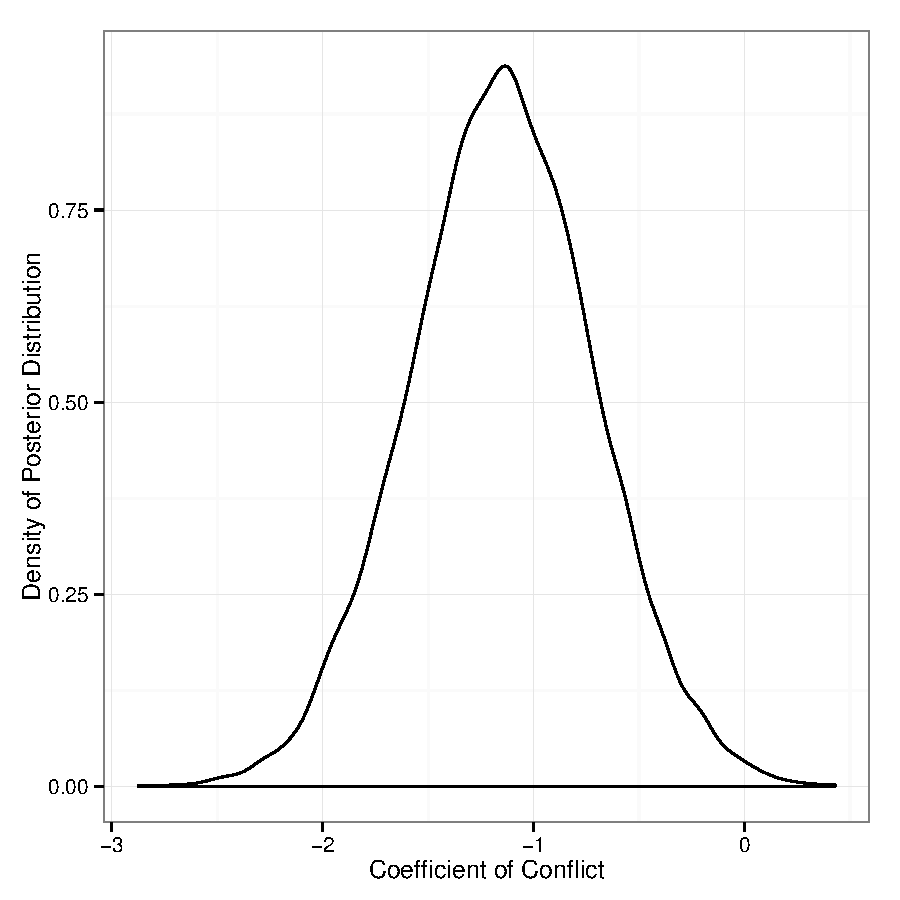
\includegraphics[width=5.25in]{Exam-f2.pdf}
  \end{center}
\end{figure}

Figure 2 plots the distribution of the Bayesian linear regression.  The distribution is centered where we would expect it, slightly negative.  This would confirm our unconditional hypothesis of the negative effect of conflict on press freedom.  However it is concerning that zero is contained by the distribution, even though it is in the far tail.  Further analysis is needed.

\pagebreak

\begin{figure}[htbp] 
  \caption{Bayesian Linear Regression Results}
  \label{F:b.conflict.plot}
  \begin{center}
    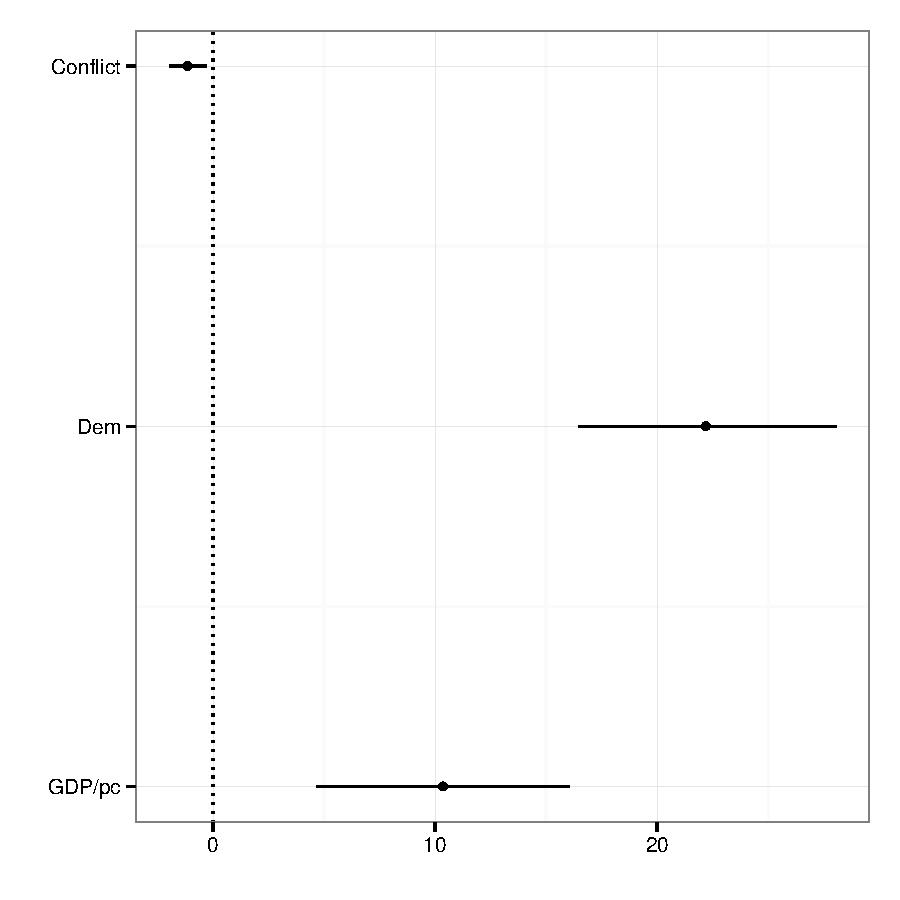
\includegraphics[width=5.25in]{Exam-f3.pdf}
  \end{center}
\end{figure}

Figure 3 plots the regression results with credible intervals.  As we can see the 95\% credible interval for the conflict variable does not include zero - the concern noted in figure 2 - this does not appear to be a problem.  We have further support for our unconditional hypothesis that higher numbers of conflict will have a negative affect on relative press freedom scores.  

\pagebreak

\item Suppose we wish to adopt a weakly informative prior that conflict has no effect on press freedom, and that we model this prior as a Cauchy distribution with location parameter 0 and scale parameter 0.5 (that is, as \verb+cauchy(0, 0.5)+).  Retain uninformative uniform priors for the control variables.  Does the posterior of a Bayesian linear regression model with these priors support the hypothesis that more conflict reduces press freedom?

\begin{Schunk}
\begin{Sinput}
> pressfree.code2 <- '
+     data {
+         int<lower=0> N;
+         vector[N] press_free;
+         vector[N] conflict;
+         vector[N] dem;
+         vector[N] gdp_pc;
+     }
+     parameters {                
+         real beta1;             // coef for constant (default prior is uniform, i.e., noninformative)
+         real beta2;             // coef for stategini
+         real beta3;
+         real beta4;
+         real<lower=0> sigma;
+     }
+     model {
+         beta1 ~ cauchy(0, 0.5);
+         beta2 ~ cauchy(0, 0.5);
+         beta3 ~ cauchy(0, 0.5);
+         beta4 ~ cauchy(0, 0.5);
+         
+         press_free ~ normal(beta1 + beta2 * conflict + beta3 * dem +
+         beta4 * gdp_pc, sigma);
+     }
+ '
> set.seed(324)
> m1.stan2.s2 <- stan(model_code = pressfree.code2, data = press2.data, 
+                 iter = 10000, chains = 3)
\end{Sinput}
\begin{Soutput}
TRANSLATING MODEL 'pressfree.code2' FROM Stan CODE TO C++ CODE NOW.
COMPILING THE C++ CODE FOR MODEL 'pressfree.code2' NOW.
cygwin warning:
  MS-DOS style path detected: C:/PROGRA~1/R/R-30~1.2/etc/x64/Makeconf
  Preferred POSIX equivalent is: /cygdrive/c/PROGRA~1/R/R-30~1.2/etc/x64/Makeconf
  CYGWIN environment variable option "nodosfilewarning" turns off this warning.
  Consult the user's guide for more details about POSIX paths:
    http://cygwin.com/cygwin-ug-net/using.html#using-pathnames
C:/Users/kellengracey/Documents/R/win-library/3.0/rstan/include//stansrc/stan/agrad/rev/var_stack.hpp:49:17: warning: 'void stan::agrad::free_memory()' defined but not used [-Wunused-function]
C:/Users/kellengracey/Documents/R/win-library/3.0/rstan/include//stansrc/stan/agrad/rev/chainable.hpp:87:17: warning: 'void stan::agrad::set_zero_all_adjoints()' defined but not used [-Wunused-function]
SAMPLING FOR MODEL 'pressfree.code2' NOW (CHAIN 1).

Iteration:    1 / 10000 [  0%]  (Warmup)
Iteration: 1000 / 10000 [ 10%]  (Warmup)
Iteration: 2000 / 10000 [ 20%]  (Warmup)
Iteration: 3000 / 10000 [ 30%]  (Warmup)
Iteration: 4000 / 10000 [ 40%]  (Warmup)
Iteration: 5000 / 10000 [ 50%]  (Warmup)
Iteration: 6000 / 10000 [ 60%]  (Sampling)
Iteration: 7000 / 10000 [ 70%]  (Sampling)
Iteration: 8000 / 10000 [ 80%]  (Sampling)
Iteration: 9000 / 10000 [ 90%]  (Sampling)
Iteration: 10000 / 10000 [100%]  (Sampling)
Elapsed Time: 1.808 seconds (Warm-up)
              1.634 seconds (Sampling)
              3.442 seconds (Total)

SAMPLING FOR MODEL 'pressfree.code2' NOW (CHAIN 2).

Iteration:    1 / 10000 [  0%]  (Warmup)
Iteration: 1000 / 10000 [ 10%]  (Warmup)
Iteration: 2000 / 10000 [ 20%]  (Warmup)
Iteration: 3000 / 10000 [ 30%]  (Warmup)
Iteration: 4000 / 10000 [ 40%]  (Warmup)
Iteration: 5000 / 10000 [ 50%]  (Warmup)
Iteration: 6000 / 10000 [ 60%]  (Sampling)
Iteration: 7000 / 10000 [ 70%]  (Sampling)
Iteration: 8000 / 10000 [ 80%]  (Sampling)
Iteration: 9000 / 10000 [ 90%]  (Sampling)
Iteration: 10000 / 10000 [100%]  (Sampling)
Elapsed Time: 2.059 seconds (Warm-up)
              2.04 seconds (Sampling)
              4.099 seconds (Total)

SAMPLING FOR MODEL 'pressfree.code2' NOW (CHAIN 3).

Iteration:    1 / 10000 [  0%]  (Warmup)
Iteration: 1000 / 10000 [ 10%]  (Warmup)
Iteration: 2000 / 10000 [ 20%]  (Warmup)
Iteration: 3000 / 10000 [ 30%]  (Warmup)
Iteration: 4000 / 10000 [ 40%]  (Warmup)
Iteration: 5000 / 10000 [ 50%]  (Warmup)
Iteration: 6000 / 10000 [ 60%]  (Sampling)
Iteration: 7000 / 10000 [ 70%]  (Sampling)
Iteration: 8000 / 10000 [ 80%]  (Sampling)
Iteration: 9000 / 10000 [ 90%]  (Sampling)
Iteration: 10000 / 10000 [100%]  (Sampling)
Elapsed Time: 1.626 seconds (Warm-up)
              1.354 seconds (Sampling)
              2.98 seconds (Total)
\end{Soutput}
\end{Schunk}

\pagebreak

\begin{Schunk}
\begin{Sinput}
> print(m1.stan2)
\end{Sinput}
\begin{Soutput}
Inference for Stan model: pressfree.code.
3 chains, each with iter=10000; warmup=5000; thin=1; 
post-warmup draws per chain=5000, total post-warmup draws=15000.

        mean se_mean  sd   2.5%    25%    50%    75%  97.5% n_eff Rhat
beta1   61.4       0 2.5   56.4   59.7   61.4   63.1   66.4  6684    1
beta2   -1.1       0 0.4   -2.0   -1.4   -1.1   -0.9   -0.3  7697    1
beta3   22.2       0 3.0   16.4   20.2   22.2   24.2   28.0  7471    1
beta4   10.4       0 2.9    4.7    8.4   10.4   12.3   16.1  8331    1
sigma   17.1       0 1.1   15.2   16.4   17.1   17.8   19.4  8944    1
lp__  -470.8       0 1.6 -474.8 -471.6 -470.4 -469.6 -468.6  5196    1

Samples were drawn using NUTS(diag_e) at Mon Mar 24 11:04:48 2014.
For each parameter, n_eff is a crude measure of effective sample size,
and Rhat is the potential scale reduction factor on split chains (at 
convergence, Rhat=1).
\end{Soutput}
\begin{Sinput}
> print(m1.stan2.s2)
\end{Sinput}
\begin{Soutput}
Inference for Stan model: pressfree.code2.
3 chains, each with iter=10000; warmup=5000; thin=1; 
post-warmup draws per chain=5000, total post-warmup draws=15000.

        mean se_mean  sd   2.5%    25%    50%    75%  97.5% n_eff Rhat
beta1   61.8     0.0 2.7   56.5   59.9   61.7   63.6   67.2  3964    1
beta2   -0.8     0.0 0.4   -1.8   -1.1   -0.8   -0.5    0.0  4944    1
beta3   22.1     0.0 3.1   16.0   20.0   22.1   24.2   28.2  4929    1
beta4    7.4     0.1 4.0   -0.2    4.6    7.7   10.3   14.5  3678    1
sigma   17.3     0.0 1.1   15.3   16.5   17.2   18.0   19.5  4834    1
lp__  -495.4     0.0 1.6 -499.3 -496.2 -495.1 -494.3 -493.3  4448    1

Samples were drawn using NUTS(diag_e) at Mon Mar 24 11:05:32 2014.
For each parameter, n_eff is a crude measure of effective sample size,
and Rhat is the potential scale reduction factor on split chains (at 
convergence, Rhat=1).
\end{Soutput}
\end{Schunk}

Looking at the two models side by side we see similar results.  However in the second model, using a weakly informative prior that conflict has no effect on press freedom, we now see a 95\% credible interval that is bound by zero (-1.8, 0.0).  Both models show a negative effect of conflict on press freedom, providing support for our hypothesis.  The second model, however, does shift the credible interval in a concerning direction (from -2.0, -0.3).  There is still somehat weak evidence supporting our unconditional hypothesis, even after adopting the subjective belief that there is no relationship.  These results are fairly robust.

\end{enumerate}
\end{document}
